%
% $LastChangedRevision: 2128 $
% $LastChangedDate:: 2021-02-02 14:38:09 +0100#$
%
% This file is part of X2C. http://x2c.lcm.at/
%
% ===== CONFIDENTIAL =====
% The content of this file is confidential according to the X2C Licence Terms and Conditions.
%
% Copyright (c) 2020, Linz Center of Mechatronics GmbH (LCM) http://www.lcm.at/
% All rights reserved.
%
For proper synchronisation with X2C timings, a \textit{Delay}-Block with SampleTimeMultiplier set to 4, must be placed infront of the "Enable" input of the block!
\begin{figure}[H]
	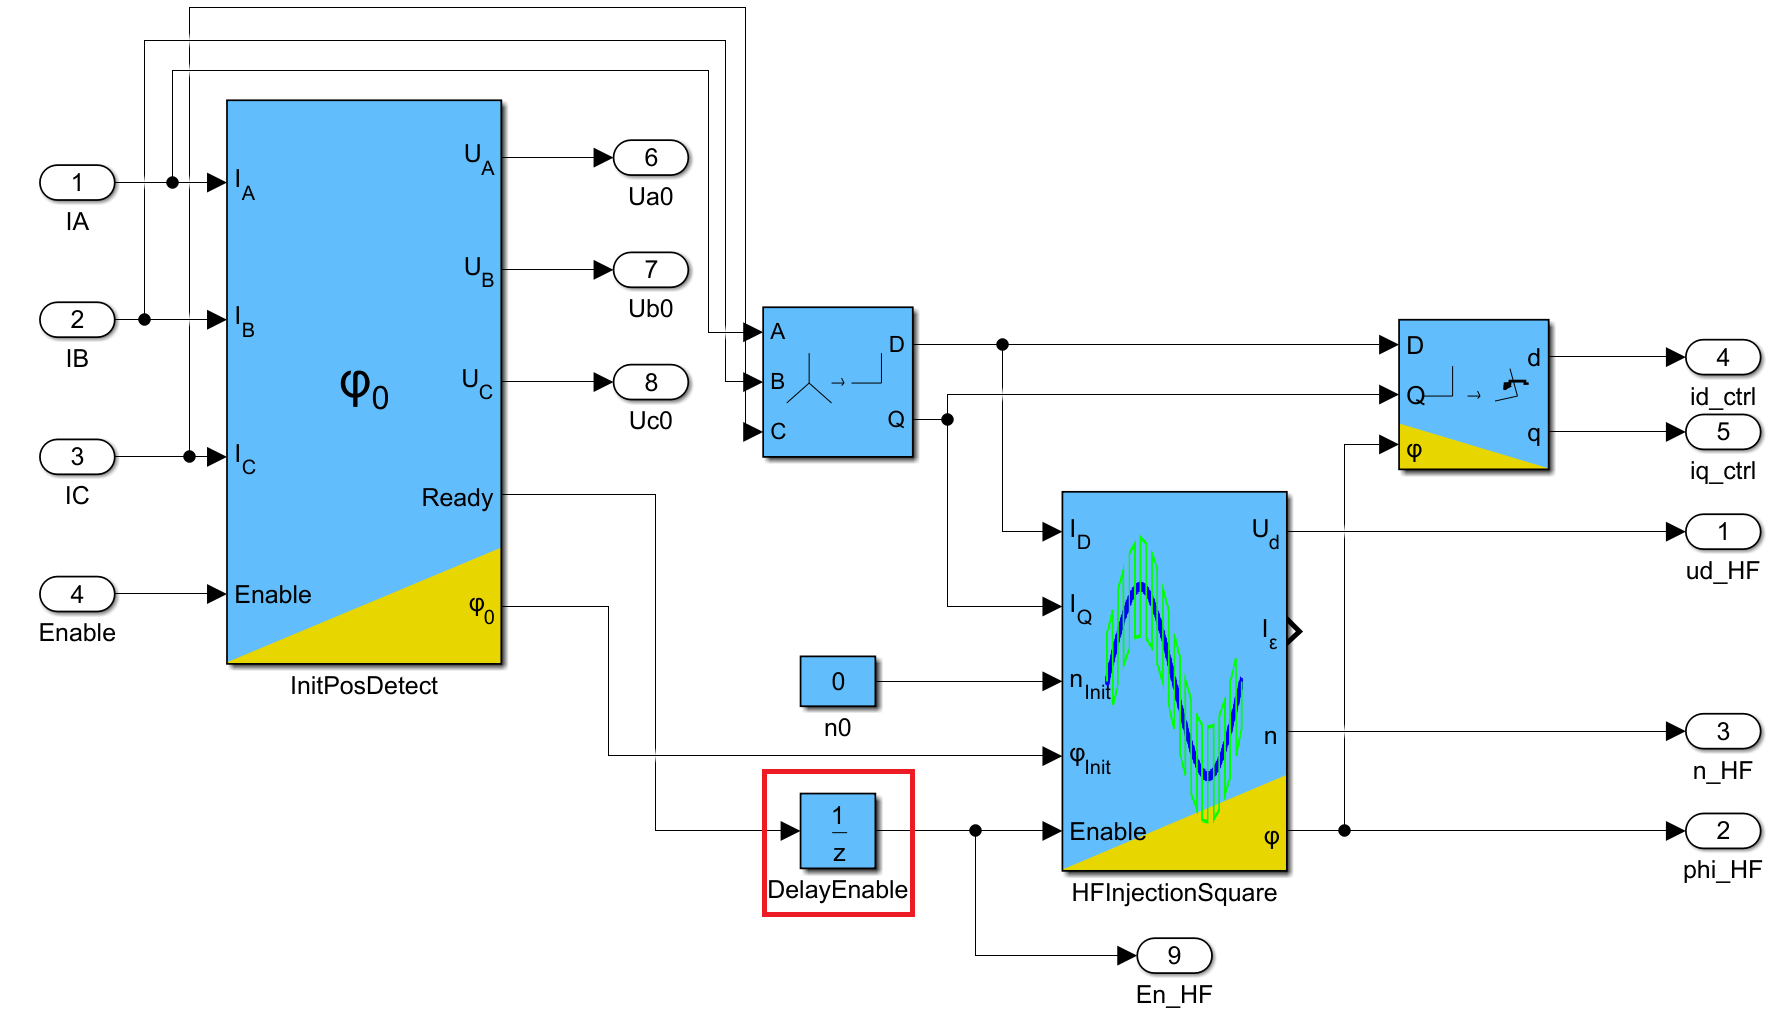
\includegraphics[width=\textwidth]{Subsystem_Sensorless_HF}
	%\label{fig:SensorlessSubsystem}
	%\caption{Sensorless Subsystem}
\end{figure}

\textbf{Procedure:}\\
The algorithm mainly spilts into two parts:
\begin{enumerate}
\item HF-Injection:\\
			This part is based on the paper \textit{"Position sensorless control of PMSM by synchronous injection and demodulation of alternating carrier voltage"} by W. Hammel and R. Kennel from 2010.\\
			A high frequent voltage is injected into the estimated flux direction $d$. The injected voltage has a constant amplitude but changes its sign with every PWM cycle. Every 4th PWM cycle a misalignment current $I_{eps}$ due to the injected voltage is calculated.\\
			The aim of the injection is getting the misalignment information when commutating using the estimated rotor angle.
\item Tracking Loop:\\
			The tracking loop calculates the rotor angle.\\
			Aim of the tracking loop is to minimize the misalignment current $I_{eps}$ with high dynamics. That way a valid estimate of the rotor angle is obtained.\\
			The block diagram of the tracking loop is shown in the figure below.\\
			The parameter of the tracking loop are chosen in a way so that the triple pole is real and negative. The step response of the loop is the same as that of three 1st order delay elements in series.\\
			The loops initial angle-value has to be provided at the block input $\varphi_{init}$. If the starting position is unknown, using the proper parameterized block {\itshape InitPosDetect} may be best. The interconnection of the blocks is shown in the figure above.
\end{enumerate}
\begin{figure}[H]
	
\includegraphics[width=\textwidth]{TrackingLoop}
	%\label{fig:trackLoop}
	%\caption{Tracking-Loop of Block \textit{HFInjectionSquare}}
\end{figure}

\paragraph{Requirement:} The motor must be salient!